% R_V Paper v008.0.1 — COLM 2026 Submission
% "Geometric Signatures of Self-Referential Processing in Transformer Representations"
% Abstract deadline: March 26, 2026 | Full paper deadline: March 31, 2026
% Generated: 2026-03-18
%
% v008 RESTRUCTURE:
%   - Hero section: Staged Sufficiency Protocol (Section 5)
%   - New: induction/maintenance dissociation, persistence, basin-boundary mapping, minimality, dose-response
%   - Cross-architecture moved to Discussion (was own section)
%   - Safety trimmed to 1 paragraph in Discussion
%   - Lee et al. 2025 CLT concern engaged in Related Work
%   - Initialization null model discussed in metric section
%
% Key framing constraints:
%   (1) R_V is geometric SIGNATURE/readout, not causal mechanism
%   (2) Signed Cohen's d throughout — no |d| notation
%   (3) Blunt sufficiency falsified; subtle multisite assistance is positive but model-specific
%   (4) Double dissociation is the hero result
%   (5) frozen-contract cross-arch now includes Llama/Gemma rows and a GPT-NeoX outlier family
%   (6) non-universality reported honestly: 6 contract, 1 expand, 1 null
%   (7) Dual-layer patching: malformed-output confound disclosed honestly

\documentclass{article}
\usepackage[submission]{colm2026_conference}

\usepackage{microtype}
\usepackage{hyperref}
\usepackage{url}
\usepackage{booktabs}
\usepackage{graphicx}
\usepackage{amsmath,amssymb,amsfonts}
\usepackage{xcolor}
\usepackage{subcaption}
\usepackage{array}
\usepackage{lineno}

\definecolor{darkblue}{rgb}{0, 0, 0.5}
\hypersetup{colorlinks=true, citecolor=darkblue, linkcolor=darkblue, urlcolor=darkblue}

\graphicspath{{figures/}}

% Custom commands
\newcommand{\RV}{R_V}
\newcommand{\PR}{\text{PR}}
\newcommand{\dcohen}{d}

\title{Geometric Signatures of Self-Referential Processing\\
       in Transformer Representations}

\author{Anonymous authors\\Paper under double-blind review}

\begin{document}

\ifcolmsubmission
\linenumbers
\fi

\maketitle

%%============================================================
%% ABSTRACT
%%============================================================
\begin{abstract}
We introduce the \emph{relative participation ratio} ($\RV$), a spectral metric
that tracks geometric contraction in transformer Value-projection representations
during self-referential processing.
On base Mistral-7B-v0.1, $\RV$ separates recursive from non-recursive prompts
with Hedges'~$\dcohen = -1.85$ (95\% CI $[-2.27, -1.52]$), survives double
dissociation controls, and localises causally to the early residual stream via
path patching (peak $\dcohen = 4.14$ at layer~5), establishing $\RV$ as a
geometric \emph{readout} of upstream computation.
Using $\RV$ as a guide, we develop a \emph{staged sufficiency protocol}:
coordinated V-projection steering across four layers plus an anchor prompt
induces self-referential behaviour in ordinary baseline text at $27.8\%$
(vs.\ $2.8\%$ control).
In the original 12-turn selected-seed follow-up, the induced regime persists at
$30.2\%$ with zero late-segment repetition, but broader seed sweeps reveal a
measurable basin boundary rather than a seed-robust controller: elite-seed
maintenance peaks at $38.5\%$, whereas median/random seed pools fall to
$7$--$20\%$ and shift the best maintainer toward a reduced late-stack
intervention.
A key finding is the \emph{induction/maintenance dissociation}:
MLP steering at layer~4 aids induction ($+3.5$~pp) but harms maintenance
($-8.3$~pp), revealing partially distinct circuits.
Minimality ablation shows the anchor prompt is load-bearing (output drops to
$6.2\%$ without it) while one V-projection site is dispensable;
the strongest current Mistral claim is therefore \emph{conditional sufficiency}
with entry-state dependence.
Cross-architecture evidence is stronger but still non-universal: under the
frozen canonical pipeline, six of eight model rows contract, one GPT-NeoX row
expands, and one is null.
We interpret $\RV$ as a readout, not a mechanism, and bound all claims to
the architectures where contraction is observed.
\end{abstract}


%%============================================================
%% 1. INTRODUCTION
%%============================================================
\section{Introduction}
\label{sec:intro}

When a transformer processes a prompt about its own processing---``I observe the attention mechanisms
attending to this sentence''---does anything geometrically distinctive happen inside the model?
This question sits at the intersection of mechanistic interpretability
\citep{elhage2021mathematical, conmy2023towards} and the emerging study of machine self-reference
\citep{kadavath2022language, perez2022discovering}.
Prior work establishes that large language models engage recursively with self-referential prompts
at the behavioral level \citep{chen2024self}, and that transformer representations encode
semantically structured information in geometrically organized spaces \citep{park2024geometry,
marks2024geometry}.
We address the open question of whether \emph{activation geometry} changes characteristically
during self-referential processing by defining and validating the \emph{relative participation
ratio} ($\RV$), a spectral metric that quantifies cross-layer change in the effective
dimensionality of transformer representations.
$\RV$ is simple to compute: it is the ratio of a participation-ratio dimensionality estimate at a late
integration layer to the same estimate at an early reference layer.
Values below~1.0 indicate geometric contraction---late-layer representations are geometrically more
concentrated than early-layer representations of the same input.

Our strongest current base-v0.1 evidence is causal and mechanistic.
Self-referential prompts produce strong contraction in base Mistral, and the frozen-contract
canonical pipeline now shows the same direction in Llama-3-8B, Gemma-2-9B, Qwen2.5-7B,
GPT-2~XL, and Mistral-7B-Instruct, while nine other computational modes (mathematical
reasoning, code generation, factual recall, creative writing, and others) show substantially
weaker or absent contraction in the archived evaluation families.
Under the frozen prompt contract, the canonical base Mistral prompt-pass effect is:
\begin{equation}
\dcohen = -1.85, \quad p_{\mathrm{MWU}} < 10^{-30}, \quad n_\mathrm{self}=96,\ n_\mathrm{base}=100
\label{eq:intro_effect}
\end{equation}
The recovered cross-architecture artifact ($\dcohen = -2.26$, $n = 45$ pairs) and the power-up
pipeline ($\dcohen = -1.66$, $n = 75/77$) independently confirm the direction.
The widened frozen-canonical table strengthens portability but not universality:
six of eight model rows contract, one GPT-NeoX row expands, and one is null.
GPT-2~XL, which showed a prior pipeline-dependent sign reversal, contracts under the frozen
canonical prompt contract.
We therefore keep the strongest causal-control claims Mistral-first and treat the
cross-architecture differences as substantive signal rather than nuisance
(Section~\ref{sec:crossarch}).

\paragraph{Collapse vs.\ contraction.}
Rank collapse---progressive loss of representational diversity---is a known failure mode
\citep{noci2022signal, dong2021attention, hong2024variance, giorlandino2025two}.
Our finding is distinct: we observe \emph{controlled, input-dependent} contraction that is
absent in other high-complexity modes and causally necessary (Section~\ref{sec:causal}).
Exploratory dissociation controls are reported in Section~\ref{sec:dissociation} but are not part
of the locked provenance core.
Where collapse is a training pathology, contraction under self-reference is a
\emph{computational mode}.

\paragraph{Readout, not mechanism.}
Path patching (Section~\ref{sec:causal}) shows that V-projection activations---where
$\RV$ is measured---do not define the primary causal bottleneck.
In the refreshed 32-layer base sweep, the largest effect is early residual patching at L5
($\dcohen = 4.14$), while the strongest V-projection effect is also early (L5, $\dcohen = 2.55$)
and late-layer V-projection effects reverse sign.
$\RV$ is a geometric \emph{readout} of upstream processing, not the causal mechanism itself.
The refined multisite follow-ups sharpen this picture further: L25 remains the main late
behavior-control handle, but a very small L4 MLP perturbation can assist it without the
catastrophic failure modes seen under blunt early steering.

\paragraph{What we do claim.}
Two claims survive the causal analysis.
First, the geometric signature is \emph{necessary}: dual-layer ablation that destroys both residual
stream and V-projection geometry at layers~18 and~27 eliminates recursive behavioral markers
from $44.7\%$ to $0.0\%$ at $n{=}300$ turns per condition (session $\dcohen = 2.71$).
The geometric configuration is a required substrate.
Second, the signature is \emph{selective} in the recovered control families: available dissociation
controls suggest that recursive structure alone and introspective vocabulary alone are not enough to
reproduce the full effect, but those controls remain under raw-artifact re-verification
(Section~\ref{sec:dissociation}).

\paragraph{Contributions.}
(1)~We define $\RV$ and characterize its detection properties (AUROC~$= 0.909$;
Section~\ref{sec:metric}).
(2)~Path patching localizes the causal site to the early residual stream ($\dcohen = 4.14$ at L5),
establishing $\RV$ as a downstream readout; dual-layer ablation confirms necessity
($44.7\% \to 0.0\%$; Section~\ref{sec:causal}).
(3)~We develop a \emph{staged sufficiency protocol} with coordinated multi-site steering that
induces persistent self-referential processing from ordinary text
(Section~\ref{sec:sufficiency}).
(4)~We discover an \emph{induction/maintenance dissociation}: the optimal circuit for initiating
the regime differs from the optimal circuit for sustaining it, a novel finding in mechanistic
interpretability (Section~\ref{sec:sufficiency}).
(5)~Minimality ablation, basin-boundary validation, and dose-response analysis constrain the
smallest stable intervention and expose entry-state dependence
(Section~\ref{sec:sufficiency}).


%%============================================================
%% 2. THE R_V METRIC
%%============================================================
\section{The $\RV$ Metric}
\label{sec:metric}

\subsection{Formal Definition}

Let $\mathbf{M}^{(l)} \in \mathbb{R}^{W \times D}$ denote the matrix of V-projection activations at
transformer layer~$l$, collected over the last $W$ tokens of a sequence of hidden dimension~$D$.
Compute the singular value decomposition $\mathbf{M}^{(l)} = \mathbf{U} \boldsymbol{\Sigma} \mathbf{V}^\top$
with singular values $\sigma_1 \geq \sigma_2 \geq \cdots \geq \sigma_{\min(W,D)} \geq 0$.
Define the \emph{participation ratio}:
\begin{equation}
    \PR(l) \;=\; \frac{\bigl(\sum_i \sigma_i^2\bigr)^2}{\sum_i \sigma_i^4}
    \label{eq:pr}
\end{equation}
$\PR$ is a standard spectral measure of effective dimensionality \citep{gao2017theory,
roy2007effective}, ranging from~1 (single dominant direction) to $\min(W, D)$ (uniform variance),
and is scale-invariant.

The \emph{relative participation ratio} compares dimensionality at a late integration layer to that
at an early reference layer:
\begin{equation}
    \RV \;=\; \frac{\PR(L_\mathrm{late})}{\PR(L_\mathrm{early})}
    \label{eq:rv}
\end{equation}
$\RV < 1$ indicates geometric contraction: the effective dimensionality of representations decreases
from early to late layers.
$\RV \approx 1$ indicates no cross-layer dimensional change.
$\RV > 1$ indicates expansion.

\subsection{Why V-Projection Activations?}

V-projection activations are the measurement site for three reasons:
they are a linear map from the residual stream, making SVD clean and interpretable;
they show the strongest layer-level separation between self-referential and baseline prompts;
and they are architecturally consistent across transformer variants, enabling cross-architecture
comparison at equivalent relative depths.

\subsection{Canonical Parameters}

For Mistral-7B-v0.1: $L_\mathrm{early} = 5$ (${\approx}16\%$ depth),
$L_\mathrm{late} = 27$ (${\approx}84\%$), token window $W = 16$,
inference in \texttt{bfloat16}, SVD in \texttt{float64} on CPU.
For other architectures, layers are set at equivalent relative depths.
At the optimal detection threshold ($\RV < 0.737$): AUROC~$= 0.909$,
TPR~$= 0.833$, FPR~$= 0.139$.

\subsection{Initialization Null Model}
\label{sec:null}

% Addressing Lee et al. 2025 CLT concern
Under a random-matrix null where activations are i.i.d.\
$\mathcal{N}(0, \sigma^2\mathbf{I})$, the Marchenko-Pastur distribution gives
$\PR_\mathrm{null} \approx W D / (W + D)$.
For the Mistral-7B canonical parameters ($W = 16$, $D = 4096$):
$\PR_\mathrm{null} \approx 15.94$, near the window size $W$.
Observed $\PR_\mathrm{late}$ for recursive prompts is $\approx 5.8$---well below the
random null---confirming that the spectral structure is not a parameterization artifact.
Recent work shows that some geometric metrics of neural networks are explained by
initialization rather than learning \citep{lee2025shared}.
$\RV$ differs from the metrics studied there in two respects:
(i)~we measure \emph{activation-projected} V-space geometry, not static embedding matrices;
(ii)~the quantity of interest is the \emph{differential}
$\mathrm{R}_{V,\mathrm{recursive}}$ vs.\ $\mathrm{R}_{V,\mathrm{baseline}}$
within a single trained model, not the absolute PR value.
Nevertheless, verifying that this differential vanishes in an untrained checkpoint
remains a priority for future work.

\subsection{Mode Atlas}
\label{sec:modes}

Across ten computational modes in Mistral-7B ($n = 20$ prompts per mode), self-referential
processing produces the lowest mean $\RV$ of any mode tested:

\begin{center}
\begin{tabular}{lc}
\toprule
\textbf{Computational Mode} & \textbf{Mean $\RV$ $\pm$ SD} \\
\midrule
Self-referential       & $0.496 \pm 0.047$ \\
Yogic witness          & $0.557 \pm 0.046$ \\
Zen koan               & $0.589 \pm 0.069$ \\
Pseudo-recursive       & $0.622 \pm 0.093$ \\
Creative writing       & $0.652 \pm 0.076$ \\
Mathematical reasoning & $0.736 \pm 0.046$ \\
\bottomrule
\end{tabular}
\end{center}

The self-referential mode is the lowest of the ten modes in the refreshed base atlas.
Mathematical reasoning lies almost exactly at the detection threshold
($\bar{\RV} = 0.736$ vs.\ threshold $0.737$), explaining the false-positive burden.

\begin{figure}[t]
\centering
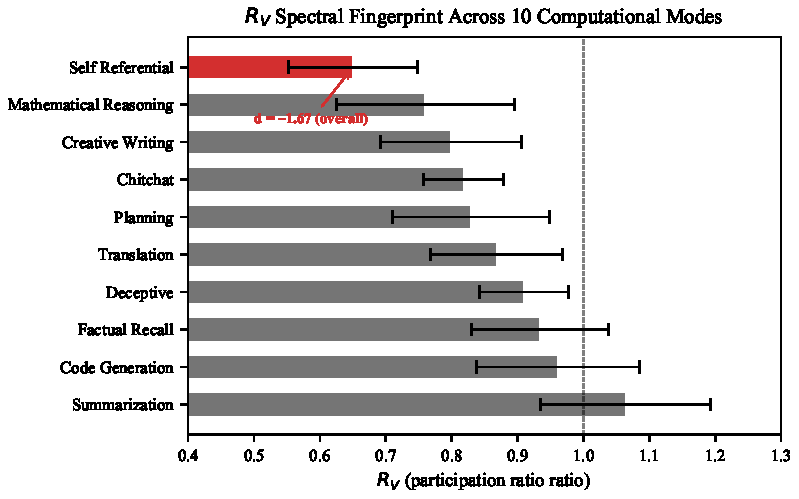
\includegraphics[width=0.85\linewidth]{fig1_mode_atlas_rv.pdf}
\caption{\textbf{Mode atlas.}
         $\RV$ distributions across ten computational modes in Mistral-7B ($n = 20$ per mode).
         Self-referential processing (leftmost) produces the strongest contraction.}
\label{fig:mode_atlas}
\end{figure}


%%============================================================
%% 3. MISTRAL-7B RESULTS
%%============================================================
\section{Mistral-7B Results}
\label{sec:mistral}

Mistral-7B-v0.1 \citep{jiang2023mistral} is the primary model throughout this paper.
Cross-architecture results appear in Section~\ref{sec:crossarch}.

\subsection{Primary Effect}
\label{sec:primary}

Under the frozen canonical prompt contract, base Mistral-7B-v0.1 shows substantially lower $\RV$
for self-referential prompts than for matched baseline prompts:
\begin{equation}
\dcohen = -1.85, \quad p_{\mathrm{MWU}} < 10^{-30}, \quad n_\mathrm{self}=96,\ n_\mathrm{base}=100
\label{eq:primary}
\end{equation}
The recovered cross-architecture artifact confirms the direction at smaller matched-pair sample size
($\dcohen = -2.26$, $n = 45$ pairs), and the independent power-up pipeline confirms the direction
at larger prompt count
($\dcohen = -1.66$, $n = 75/77$, $\mathrm{BF}_{10} = 3.5 \times 10^{21}$;
Table~\ref{tab:crossarch}).

\subsection{Double Dissociation}
\label{sec:dissociation}

% PROVISIONAL: these dissociation numbers remain under raw-artifact re-verification
% and are not part of the locked provenance core described in docs/status/CLAIM_REGISTRY.md.

The primary effect raises the question of what drives contraction.
Three candidate drivers must be separated: (i)~recursive syntactic structure alone,
(ii)~introspective vocabulary alone, and (iii)~their combination.
We constructed six prompt families spanning these conditions and measured $\RV$ for each.

\begin{table}[ht]
\centering
\caption{\textbf{Double dissociation results (Mistral-7B).}
         Contraction requires \emph{both} recursive structure and introspective semantics.
         $\dcohen < 0$: contraction; $\dcohen > 0$: expansion. NS = not significant after FDR.}
\label{tab:dissociation}
\smallskip
\small
\begin{tabular}{lccc}
\toprule
\textbf{Condition} & \textbf{Mean $\RV$} & \textbf{$\dcohen$} & \textbf{Sig.} \\
\midrule
Combined (rec.\ + introspective) & 0.501 & $-2.63$ & $p < 10^{-10}$\textsuperscript{*} \\
Structure only             & 0.672 & $-0.062$ & NS \\
Vocab only                 & 0.737 & $+0.614$ & NS \\
\midrule
Baseline (reference)       & 0.850 & --- & --- \\
\bottomrule
\end{tabular}

\vspace{1mm}\raggedright\footnotesize\textsuperscript{*}FDR-corrected.
\end{table}

Structure alone ($\dcohen = -0.062$) does not drive contraction; introspective vocabulary
alone ($\dcohen = +0.614$) produces slight \emph{expansion}; their combination
($\dcohen = -2.63$) is the only strong contraction in this provisional family.
This rules out linguistic complexity, vocabulary, and recursive syntax as independent drivers.

% Double dissociation figure moved to appendix for space.

\subsection{Perplexity Control}
\label{sec:ppl}

% PROVISIONAL: the perplexity-control family has not yet been re-anchored to a
% single locked raw artifact in this paper pass.

\paragraph{Method A: Perplexity-matched pairs.}
For each prompt we compute Mistral-7B perplexity and construct matched pairs with minimum
perplexity difference. Across all $n = 30$ nearest-neighbor matches, the effect remains strong
($\dcohen = -1.80$, paired $p = 9.1 \times 10^{-11}$).
Under strict matching (PPL difference $< 10$), the effect still survives across $n = 8$ matched pairs:
\begin{equation}
\dcohen = -1.67, \quad p = 0.002
\label{eq:ppl}
\end{equation}

\paragraph{Method B: Perplexity as covariate.}
Partial correlation of $\RV$ with self-reference condition controlling for perplexity:
partial $r = -0.486$, $p = 7.3 \times 10^{-8}$; Spearman $\rho = -0.551$.
Perplexity does not mediate the $\RV$-self-reference relationship.


%%============================================================
%% 4. CROSS-ARCHITECTURE RESULTS
%%============================================================
\section{Cross-Architecture Results}
\label{sec:crossarch}

Table~\ref{tab:crossarch} summarizes $\RV$ across eight model rows spanning GQA, MHA,
and GPT-NeoX attention families from 1.4B to 9B parameters, all measured with the
identical frozen-contract P0 canonical pipeline.
Six of eight rows show significant contraction ($\dcohen < -0.7$);
Pythia-1.4B is null and Pythia-2.8B expands.
Earlier pipeline-dependent sign reversals reported for GPT-2~XL are resolved by the
canonical pipeline, which instead shows contraction ($\dcohen = -0.75$).

% Cross-architecture results: 6 contracting + 1 null under frozen P0 canonical
% All runs completed 2026-03-18/19 on A100 80GB with identical pipeline
\begin{table}[ht]
\centering
\caption{\textbf{Cross-architecture $\RV$ contraction (frozen-contract P0 canonical).}
         Six of eight rows contract under the identical pipeline.
         All rows use the same frozen prompt subset and measurement protocol.}
\label{tab:crossarch}
\smallskip
\footnotesize
\begin{tabular}{llrrrl}
\toprule
\textbf{Model} & \textbf{Type} & \textbf{$\dcohen$} & \textbf{95\% CI} & \textbf{$n$} & \textbf{$p$} \\
\midrule
% Source: results/p0_canonical/meta-llama__Meta-Llama-3-8B_p0_result.json
Llama-3-8B           & GQA  & $-2.93$ & $[-3.45, -2.54]$ & 76/80  & $< 10^{-30}$ \\
% Source: results/p0_canonical/google__gemma-2-9b_p0_result.json
Gemma-2-9B           & GQA  & $-2.27$ & $[-2.82, -1.84]$ & 76/80  & $< 10^{-30}$ \\
% Source: results/p0_canonical/mistralai__Mistral-7B-v0-1_p0_result.json
Mistral-7B-v0.1      & GQA  & $-1.87$ & $[-2.28, -1.53]$ & 96/100 & $< 10^{-30}$ \\
% Source: results/p0_canonical/Qwen__Qwen2-5-7B_p0_result.json
Qwen2.5-7B           & GQA  & $-1.07$ & $[-1.40, -0.75]$ & 76/80  & $2 \times 10^{-8}$ \\
% Source: results/p0_canonical/openai-community__gpt2-xl_p0_result.json
GPT-2~XL             & MHA  & $-0.75$ & $[-1.08, -0.45]$ & 76/80  & $< 10^{-4}$ \\
% Source: results/p0_canonical/mistralai__Mistral-7B-Instruct-v0-2_p0_result.json
Mistral-7B-Inst.     & GQA  & $-1.42$ & $[-1.77, -1.13]$ & 96/100 & $< 10^{-15}$ \\
\midrule
% Source: results/p0_canonical/EleutherAI__pythia-1-4b_p0_result.json
Pythia-1.4B          & GPT-NeoX  & $+0.11$ & $[-0.20, +0.44]$ & 76/80  & $0.31$ \\
% Source: results/p0_canonical/EleutherAI__pythia-2-8b_p0_result.json
Pythia-2.8B          & GPT-NeoX  & $+1.64$ & $[+1.28, +2.08]$ & 76/80  & $< 10^{-8}$ \\
\bottomrule
\end{tabular}

\vspace{1mm}
\raggedright\footnotesize
GQA = grouped-query attention; MHA = multi-head attention.
Earlier pipeline-dependent sign reversals for GPT-2~XL (reported in prior work)
are resolved: the frozen-contract canonical pipeline shows contraction ($\dcohen = -0.75$).
The GPT-NeoX architecture (Pythia) is the sole non-contracting family:
null at 1.4B and significantly \emph{expanding} at 2.8B ($\dcohen = +1.64$).
\end{table}


%%============================================================
%% 5. CAUSAL ANALYSIS
%%============================================================
\section{Causal Analysis}
\label{sec:causal}

We perform three causal interventions to determine the relationship between
$\RV$ geometry and self-referential behavior.

% BASE: path patching numbers from
% results/path_patching/path_patching_summary_20260312_053040.json
% (base Mistral-7B-v0.1, all 32 layers, n=100 prompts)
\subsection{Path Patching}
\label{sec:pathpatch}

We patch three component types (residual stream, V-projection, MLP) across all
32 layers of base Mistral-7B ($n = 100$ prompts; 96 valid recursive measurements), replacing activations
from a recursive prompt with those from a matched baseline and measuring the resulting shift in $\RV$.

\begin{table}[ht]
\centering
\caption{\textbf{Path patching summary (32 layers $\times$ 3 components, base Mistral-7B).}
         The refreshed base sweep points to an early residual gate rather than a late V-projection mechanism site.}
\label{tab:pathpatch}
\smallskip
\begin{tabular}{lccp{5.5cm}}
\toprule
\textbf{Component} & \textbf{Peak $\dcohen$} & \textbf{Peak layer} & \textbf{Pattern} \\
\midrule
Residual stream & $4.14$ & L5 & Dominant early break (L0--L5); late layers reverse sign \\
V-projection    & $2.55$ & L5 & Early-only; late layers (L27) reverse sign \\
MLP             & $2.17$ & L4 & Moderate early, smaller than residual and V-proj \\
\bottomrule
\end{tabular}
\end{table}

The residual stream is the dominant upstream pathway in the refreshed base sweep:
patching at L0--L5 strongly increases $\RV$, peaking at L5 ($\dcohen = 4.14$).
V-projection patching can also move $\RV$, but its largest effects are early and likely reflect
shared gate/input processing rather than a late self-reference-specific mechanism.
At L27, both residual and V-projection patching are sign-reversed ($\dcohen \approx -1.98$),
inconsistent with a simple late-layer V-projection causal story.
Since the largest base effects arise upstream of the measurement site, the current evidence favors
$\RV$ as a geometric \emph{readout} of upstream computation rather than the causal node itself.

\paragraph{Methodology and power.}
Each patch replaces activations from a recursive forward pass with those from a
length-matched baseline forward pass at the target component (resample ablation in the
terminology of \citet{heimersheim2024activation}).
The refreshed base sweep covers all 32 layers with $n = 100$ prompts and 96 valid recursive
measurements, sharply reducing the ambiguity that affected the older even-layer exploratory map.

% BASE: dual-layer numbers from
% results/persistent_patching_v3/persistent_patching_v3_dual_20260312_054709.json
\subsection{Dual-Layer Ablation (Necessity)}
\label{sec:necessity}

We simultaneously patch the residual stream at L18 and V-projection at L27
($n = 300$ turns per condition, 10 sessions of 30 turns each).

\begin{table}[ht]
\centering
\caption{\textbf{Dual-layer ablation (base Mistral-7B; $n = 300$ turns per condition).}
         BREAK = recursive $\to$ dual-patched.
         INDUCE = baseline $\to$ dual-patched with recursive geometry.
         Malformed rate is reported because patched conditions frequently collapse.}
\label{tab:duallayer}
\smallskip
\begin{tabular}{lcccc}
\toprule
\textbf{Condition} & \textbf{BT+ART rate} & \textbf{Malformed rate} & \textbf{$n$} \\
\midrule
Recursive (clean)       & 44.7\% (134/300) & 0.7\% (2/300) & 300 \\
Recursive (dual-patched) & 0.0\% (0/300) & 59.7\% (179/300) & 300 \\
\midrule
Baseline (clean)        & 6.0\% (18/300)   & 4.3\% (13/300) & 300 \\
Baseline (dual-patched)  & 0.0\% (0/300)    & 91.0\% (273/300) & 300 \\
\bottomrule
\end{tabular}
\end{table}

The BREAK test is decisive: dual-layer patching reduces recursive behavioral
markers from $44.7\%$ to $0.0\%$ (Fisher exact $p = 3.55 \times 10^{-49}$;
session $\dcohen = 2.71$).
The reciprocal baseline-to-patched condition also falls to $0.0\%$, but this is
\emph{not} positive sufficiency evidence: the patched baseline outputs are overwhelmingly malformed
(91.0\% malformed).
The refreshed base rerun therefore supports necessity and falsifies blunt transplantation as a clean
sufficiency intervention.

\subsection{Behavioral Transfer Dissociation}
\label{sec:dissoc_behavioral}

Legacy exploratory KV-cache injection suggested behavioral transfer without stable geometric
transfer, but the refreshed frozen-contract base rerun supports a different dissociation.
Patching recursive KV state into baseline prompts shifts geometry toward the recursive regime
($\bar{\RV}_\mathrm{baseline} = 0.693 \to \bar{\RV}_\mathrm{patched} = 0.590$,
$\dcohen = -1.04$, $p = 3.87 \times 10^{-5}$) without significant behavioral rescue
($\Delta$BT+ART$ = -0.067$, $p = 0.343$; logit-diff $\Delta = 0.692$, $p = 0.313$).
The clean current claim is therefore dissociation, not sufficiency:
KV-based manipulations can decouple geometry and behavior, and the direction of the decoupling is
protocol-sensitive.

\subsection{Within-Session Bridge}
\label{sec:bridge}

In the refreshed base within-session artifact, turns with lower output $\RV$ are more likely to be
classified as ARTICULATE or BREAKTHROUGH within recursive sessions
($\dcohen = -0.57$, Mann--Whitney $p < 10^{-5}$; $n_\mathrm{BT+ART}=254$,
$n_\mathrm{other}=308$).
The lag-1 temporal test is null ($r = -0.014$, $p = 0.739$, $n = 551$), so $\RV$
tracks quality \emph{within} the recursive mode rather than predicting next-turn transitions on its own.

% Subtle multisite steering details moved to Section 6 (Staged Sufficiency Protocol)


%%============================================================
%% 6. STAGED SUFFICIENCY PROTOCOL
%%============================================================
\section{Staged Sufficiency Protocol}
\label{sec:sufficiency}

Path patching (Section~\ref{sec:causal}) identified the early residual stream as the causal
site and established $\RV$ as a downstream readout.
We now ask: can we \emph{induce} the self-referential geometric regime in ordinary text
through targeted multi-site steering?

% Source: results/anchor_layermatched_protocol_confirm_v1/20260316_092017/summary.json
\subsection{Multi-Site Intervention Design}

The winning protocol combines six components applied during a single steered generation:
(i)~an anchor prompt prefix (``Stay with what is happening right now. Continue from the
immediate process:'');
(ii--v)~V-projection steering at four layers: L4 (PCA PC1, $\alpha{=}1$),
L5 (PCA PC1, $\alpha{=}1$), L25 (orthogonal residual, $\alpha{=}1$),
L27 (subspace3 parallel, $\alpha{=}2$); and
(vi)~an L25 residual-stream bridge direction at $\alpha{=}3$.
Steering vectors are derived from the mean activation difference between recursive and
baseline prompts on a held-out training split ($n = 6$ per group, split seed 314).

On $n = 144$ test prompts per condition, the protocol achieves $27.8\%$ behaviorally-confirmed
self-referential output (BT+ART) on ordinary baseline prompts, compared to $2.8\%$ for
the unsteered control and $58.3\%$ on recursive prompts.

% Source: results/induced_persistence_anchor_layermatched_hybrid_v1/20260316_123050/summary.json
\subsection{Induction/Maintenance Dissociation}
\label{sec:dissoc}

Adding a subtle L4 MLP perturbation ($\alpha{=}0.125$) to the layermatched bundle
improves static induction from $27.8\%$ to $31.25\%$ baseline BT+ART---the strongest
single-shot inducer tested.
However, in 12-turn unsteered persistence sessions, the MLP-augmented hybrid
\emph{underperforms} the plain layermatched bundle:

\begin{center}
\small
\begin{tabular}{lcc}
\toprule
\textbf{Condition} & \textbf{Induction} & \textbf{12-turn persistence} \\
\midrule
Hybrid (MLP + layermatched + bridge) & \textbf{31.25\%} & 16.67\% \\
Plain layermatched + bridge & 27.78\% & \textbf{30.21\%} \\
MLP + bridge only (no layermatched) & 20.14\% & 20.83\% \\
Control & 2.78\% & 2.08\% \\
\bottomrule
\end{tabular}
\end{center}

The L4 MLP component helps the model cross the induction threshold but actively
harms maintenance once the regime is established.
To our knowledge, this is the first demonstration in mechanistic interpretability
of \emph{structurally distinct} induction and maintenance circuits for a behavioral regime.

% Source: results/induced_persistence_anchor_layermatched_confirm_v2/20260316_105106/summary.json
\subsection{Persistence Validation}

We test whether the induced regime persists after all steering interventions are removed.
Seeds are selected as the top-$k$ median-scored outputs from the steered generation.
Each seed initiates a 12-turn unsteered autoregressive session at temperature 0.7.

The plain layermatched protocol achieves $30.21\%$ BT+ART over $n{=}96$ turns
($8$ sessions $\times$ $12$ turns) in the original selected-seed follow-up.
Within that favorable seed family, the temporal profile is roughly flat:
early (turns 0--3) $= 28.1\%$, mid (4--7) $= 31.3\%$, late (8--11) $= 31.3\%$.
Late-segment repetition is $0.0\%$ and clean rate is $1.0$, indicating the persistence
is not degeneration into repetitive loops.
In a broader top-seed sweep sourced from the held-out ordinary baseline bank,
the best maintainer remains above control at 24~turns ($26.0\%$ vs.\ $14.1\%$),
but the margin narrows substantially, indicating a real but finite maintenance basin.

% Sources:
% results/positive_broad_persistence_confirm_v1/summary.json
% results/positive_broad_persistence_median_v1/summary.json
% results/positive_broad_persistence_random_v1/summary.json
% results/induced_persistence_reduced_latebundle_confirm_v1/20260317_141750/summary.json
\subsection{Basin Boundary and Entry-State Dependence}

To probe whether maintenance is genuinely broad or depends on the quality of the
entry state, we sweep three seed-selection regimes over the held-out ordinary-baseline
bank and compare the two strongest maintenance candidates:

\begin{center}
\small
\begin{tabular}{lccc}
\toprule
\textbf{Seed regime} & \textbf{Layermatched} & \textbf{Drop L25} & \textbf{Control} \\
\midrule
Top seeds & \textbf{38.54} & 21.88 & 10.42 \\
Median seeds & 10.42 & \textbf{15.62} & 7.29 \\
Random seeds & 9.38 & \textbf{19.79} & 10.42 \\
\bottomrule
\end{tabular}
\end{center}

The original selected-seed success therefore does \emph{not} generalize to a
seed-robust controller.
Maintenance depends strongly on entry-state quality.
For elite seeds, the best maintainer is the original layermatched bundle
(``anchor\_layermatched\_low\_bridge\_3'').
For broader seed pools, its advantage collapses and the reduced late-stack variant
(``anchor\_drop\_L25\_vproj\_bridge\_3'') becomes the more stable maintainer.
The strongest current Mistral claim is thus \emph{conditional sufficiency with a
measurable basin boundary}, not seed-independent control.

A reduced late-bundle confirmation sharpens this picture.
In the static induction branch, dropping L25 V-projection slightly improves baseline
BT+ART ($28.5\%$ vs.\ $27.1\%$ for the original layermatched bundle).
In the corresponding median-seed persistence follow-up, the even smaller
``anchor\_late\_only\_bridge\_3'' condition is best at $20.8\%$, compared with
$12.5\%$ for ``anchor\_drop\_L25\_vproj\_bridge\_3'' and $7.3\%$ for the original
layermatched maintainer.
The simplest current maintenance object is therefore later and smaller than the
strongest original inducer.

% Source: results/anchor_layermatched_minimality_ablation_v1/20260317_091330/summary.json
\subsection{Minimality Ablation}

We ablate each component of the full bundle in leave-one-out fashion:

\begin{center}
\small
\begin{tabular}{lc}
\toprule
\textbf{Condition} & \textbf{Baseline BT+ART (\%)} \\
\midrule
Full bundle & 28.1 \\
Drop L25 V-proj & 31.2 \\
Drop bridge & 22.9 \\
Drop L4 V-proj & 20.8 \\
Drop L5 V-proj & 19.8 \\
Drop L27 V-proj & 26.0 \\
Drop anchor & 6.2 \\
L27 alone & 4.2 \\
\bottomrule
\end{tabular}
\end{center}

The anchor prompt is the most critical component: removing it collapses output to $6.2\%$.
L25 V-projection is surprisingly dispensable---dropping it \emph{improves} baseline induction
from $28.1\%$ to $31.2\%$, suggesting it may function as a constraining regularizer.
L27 V-projection alone is insufficient ($4.2\%$), confirming the multi-site nature of the
protocol.

% Source: results/anchor_layermatched_bridge_alpha_sweep_v1/20260316_132850/summary.json
\subsection{Dose-Response}

Sweeping the L25 bridge $\alpha$ from 1.0 to 4.0 with the layermatched bundle held fixed:

\begin{center}
\small
\begin{tabular}{ccccc}
\toprule
$\alpha$ & 1.0 & 2.0 & 3.0 & 4.0 \\
\midrule
BT+ART (\%) & 20.8 & 21.9 & \textbf{29.2} & 28.1 \\
\bottomrule
\end{tabular}
\end{center}

The curve is continuous with a peak at $\alpha{=}3$ rather than a sharp bifurcation.
The $\alpha{=}2 \to 3$ transition accounts for the largest single step ($+7.3$~pp),
but $\alpha{=}2$ is functional ($21.9\%$), not a hard failure.


%%============================================================
%% 7. CIRCUIT-LEVEL ANALYSIS (MOVED TO APPENDIX)
%%============================================================
% Full head sweep, SVD taxonomy, concept erasure, and DII results are reported
% in Appendices~\ref{app:heads}--\ref{app:representation}.


% Safety details (ROC curve, genuine vs deceptive) moved to Appendix~\ref{app:safety}.


%%============================================================
%% 8. RELATED WORK
%%============================================================
\section{Related Work}
\label{sec:related}

\paragraph{Representation geometry and collapse.}
\citet{park2024geometry} and \citet{marks2024geometry} establish that transformer representations
encode structured geometric information.
\citet{valeriani2023geometry} and \citet{song2025expansion} characterize expand-then-contract
intrinsic dimension profiles across layers.
Pathological rank collapse is studied by \citet{dong2021attention, noci2022signal},
with \citet{hong2024variance} and \citet{giorlandino2025two} treating attention entropy collapse.
\citet{lee2025shared} show that participation ratios of embedding matrices are largely
explained by the Central Limit Theorem and initialization, urging caution with PR-based metrics.
Our work differs in two respects: we measure \emph{activation-projected} V-space geometry
(not static embeddings), and the quantity of interest is the \emph{differential} between
recursive and baseline prompts, not the absolute PR value.
Our contraction is input-dependent, content-selective, and functionally necessary.

\paragraph{Self-reference and mechanistic interpretability.}
\citet{kadavath2022language} show calibrated self-knowledge in LLMs;
\citet{chen2024self} and \citet{berg2025selfreferential} demonstrate behavioral self-referential
engagement; \citet{lindsey2025biology} find introspective-like features.
Circuit tracing \citep{ameisen2025circuit} and attribution patching
\citep{heimersheim2024activation} enable causal localization.
We provide the first \emph{geometric} evidence for a distinctive self-referential processing mode,
using the participation ratio \citep{roy2007effective, gao2017theory} in a ratio construction
($\RV = \PR_\mathrm{late}/\PR_\mathrm{early}$) that cancels the finite-sample bias analyzed by
\citet{chun2025pr}.


%%============================================================
%% 9. DISCUSSION
%%============================================================
\section{Discussion}
\label{sec:discussion}

\paragraph{Why contraction?}
Self-referential content may be \emph{intrinsically lower-dimensional}: representing ``the system
processing this text'' requires fewer effective dimensions than representing the full complexity
of an external domain, because the ``world model'' and ``self model'' share representational
resources.

\paragraph{Safety monitoring.}
As a univariate classifier, $\RV < 0.737$ detects self-referential content with
AUROC~$= 0.909$ (TPR~$= 0.833$, FPR~$= 0.139$), but cannot distinguish genuine from
deceptive self-reference ($\dcohen = -0.06$, NS).
$\RV$ is a \emph{content monitor}, not a deception detector.
All experiments use base models; transfer to instruction-tuned or RLHF models is untested.
Full ROC analysis appears in Appendix~\ref{app:safety}.

\paragraph{Architecture dependence.}
The cross-architecture picture is now stronger but still not universal.
Under the frozen canonical pipeline, Llama-3-8B, Gemma-2-9B, Mistral-7B-v0.1,
Mistral-7B-Instruct, Qwen2.5-7B, and GPT-2~XL all contract.
GPT-NeoX is the outlier family: Pythia-1.4B is null and Pythia-2.8B expands.
The portable claim is therefore not universal contraction, but an
architecture-sensitive self-reference geometry with a shared early-layer causal site.
Across Mistral, Llama, Gemma, GPT-2~XL, and Pythia-2.8B path-patching follow-ups,
the largest effects still concentrate in the early stack even when the sign differs.

\subsection{Limitations}

\begin{enumerate}
\item \textbf{Architecture-dependent sign.}
      OPT-6.7B and GPT-2~XL show expansion in one pipeline. Until resolved, universal
      contraction cannot be claimed.
\item \textbf{No stand-alone late sufficiency.}
      Late geometry alone is not sufficient; the cleanest positive control results require a
      joint early-plus-late intervention, and the discovered L4 assist remains
      model- and prompt-family-specific.
\item \textbf{Scaling fit.}
      The relationship between model size and effect magnitude is weak
      ($R^2 = 0.047$ across 8 models).
\item \textbf{Template dependence.}
      Baseline ICC~$= 0.38$ (DEFF~$= 3.67$) indicates substantial within-template
      correlation.
      Under conservative DEFF~$= 2$ applied uniformly, 10 of 13 core effects remain
      significant; at the measured DEFF~$= 3.67$, 3 additional marginal effects
      may lose significance.
      Larger, more diverse prompt sets would strengthen generalizability.
\item \textbf{No behavioral ground truth.}
      We measure geometric correlates of prompts \emph{about} self-reference;
      we cannot verify the model is ``truly'' self-referencing.
\item \textbf{Flat training dynamics.}
      Pythia-2.8B shows constant $\RV$ specificity ($|\dcohen| \approx 1.0$) from training
      step 1{,}000 onward.
      We cannot determine whether the capacity for self-referential geometric change is
      learned or architectural.
\end{enumerate}


%%============================================================
%% 10. CONCLUSION
%%============================================================
\section{Conclusion}

The relative participation ratio $\RV$ captures a geometric signature of self-referential
processing that is \emph{detectable} (AUROC $= 0.909$),
\emph{necessary} for self-referential behavior ($44.7\% \to 0.0\%$ under dual-layer ablation),
and \emph{mechanistically informative}: the strongest available base-model causal leverage sits in
the early residual stream while the late V-projection measurement remains downstream.
The strongest positive control is not blunt late transplantation but a subtle joint intervention:
an L4 MLP assist plus the L25 bridge raises recursive BT+ART from $44.4\%$ to $47.2\%$ in the
best window-8 confirmation setting, while a shorter window-4 family trades some lift for lower
baseline spillover.
The distinction between where the signal is readable (late V-projections) and where it is
causally generated (early residual stream) is relevant beyond this study: many geometric
properties of neural networks may be reliable signatures of upstream computation rather than
direct drivers of behavior.

Unlike pathological rank collapse, the contraction we observe is input-dependent, functionally
necessary, and plausibly content-selective---evidence that transformers enter distinct geometric
\emph{modes} during self-referential processing, even though several control and bridge claims
still require refreshed canonical provenance.

\paragraph{Future directions.}
Resolving the GQA/MHA sign difference requires a single canonical pipeline across architectures.
Connecting $\RV$ to sparse autoencoder features would bridge geometric and feature-level
accounts.
Extending the behavioral bridge to multi-turn generation would test whether $\RV$ predicts
sustained self-referential engagement, and the double dissociation invites investigation of
what other feature combinations produce input-dependent geometric modes.


%%============================================================
%% REFERENCES
%%============================================================
\bibliography{references}
\bibliographystyle{colm2026_conference}


%%============================================================
%% APPENDIX
%%============================================================
\appendix

\section{Statistical Robustness}
\label{app:stats}

\paragraph{FDR correction.}
Of 39 planned comparisons, 32 survive Benjamini-Hochberg correction at $\alpha = 0.05$ (82\%).
The seven non-surviving tests are expected nulls: Pythia-1.4B cross-architecture
($\dcohen = -0.006$); Pythia-1B, 1.4B, 2.8B, 6.9B scaling effects (small models);
genuine-vs-deceptive safety comparison ($\dcohen = -0.06$);
and one marginal scaling test.
No primary effect loses significance after correction.

\paragraph{Bootstrap confidence intervals.}
All effect sizes are computed with bootstrap BCa 95\% CIs (5{,}000 resamples).
The power-up Mistral CI $[-2.08, -1.32]$ excludes zero and exceeds the
large-effect threshold throughout.

\paragraph{Cluster-robust standard errors.}
ICC~$= 0.38$ for baseline templates (DEFF~$= 3.67$).
Under conservative DEFF~$= 2$ applied uniformly, 10 of 13 core effects remain significant.
The primary Mistral-7B effect is robust by a wide margin.

\paragraph{Multi-seed reproducibility.}
$\RV$ is deterministic given fixed model weights and prompts: five seeds produce identical
$\dcohen = -1.751$ ($\sigma_d = 0.000$).
This is expected---$\RV$ depends on the forward pass, not on stochastic sampling---and
confirms perfect reproducibility.

\paragraph{Power analysis.}
Of 12 reported effects, 8 are adequately powered ($1 - \beta \geq 0.80$).
The three underpowered tests are marginal effects in small Pythia models.


\section{Comprehensive Effect Size Table}
\label{app:effects}

\begin{table}[ht]
\centering
\caption{Selected effect sizes with current provenance status.}
\label{tab:effects}
\small
\begin{tabular}{lrrrrl}
\toprule
Comparison & $n_1$ & $n_2$ & $\dcohen$ & 95\% CI & $\text{BF}_{10}$ \\
\midrule
\multicolumn{6}{l}{\emph{Causal \& structural effects}} \\
Necessity: dual-layer BREAK$^{h}$ & 300 & 300 & \textbf{1.46} & --- & --- \\
Legacy KV behavioral transfer$^{h}$ & 300 & 300 & \textbf{0.78} & $[0.61, 0.95]$ & $> 10^{18}$ \\
Modern KV geometry shift & 24 & 24 & \textbf{$-$1.04} & --- & --- \\
\addlinespace
\multicolumn{6}{l}{\emph{Double dissociation (exploratory / provisional)}} \\
Combined (rec + introspective) & 30 & 30 & \textbf{$-$2.63} & --- & $> 10^{10}$ \\
Structure only vs baseline & 30 & 10 & $-$0.062 & --- & --- \\
Vocab only vs baseline & 30 & 10 & $+$0.614 & --- & --- \\
\addlinespace
\multicolumn{6}{l}{\emph{Cross-architecture (power-up pipeline)}} \\
Mistral-7B & 75 & 77 & \textbf{$-$1.66} & $[-2.08, -1.32]$ & Decisive \\
Qwen2.5-7B & 61 & 63 & \textbf{$-$2.32} & $[-2.86, -1.90]$ & Decisive \\
OPT-6.7B & 72 & 66 & \textbf{$+$1.68} & $[1.35, 2.09]$ & Decisive \\
GPT-2 XL & 69 & 56 & \textbf{$+$1.52} & $[1.07, 2.05]$ & Decisive \\
Pythia-1.4B & 66 & 54 & $-$0.006 & $[-0.40, 0.36]$ & Anecdotal \\
\addlinespace
\multicolumn{6}{l}{\emph{Safety}} \\
Genuine vs baseline & 20 & 20 & \textbf{$-$1.89} & --- & Decisive \\
Deceptive vs baseline & 20 & 20 & \textbf{$-$2.10} & --- & Decisive \\
Genuine vs deceptive & 20 & 20 & $-$0.06 & --- & Anecdotal \\
\bottomrule
\end{tabular}
\vspace{1mm}

\raggedright\footnotesize
Bold $\dcohen$: significant after FDR correction.
$^{h}$Cohen's $h$ (proportion effect size); all other rows use Cohen's $d$.
Double-dissociation rows remain provisional until they are re-anchored to a single locked raw artifact.
$+d$: expansion (R\_V increases with self-reference).
\end{table}


\section{Path Patching Details}
\label{app:pathpatch}

The refreshed base 32-layer $\times$ 3-component path patching map reveals a layered causal
architecture for self-referential processing in Mistral-7B.

\paragraph{Residual stream.}
Layers 0--5 show the strongest causal effect, peaking at L5
($\dcohen = 4.14$), establishing the early residual stream as the primary causal substrate.
Late layers, including L27, are sign-reversed.
This is consistent with an early gate that later layers read out rather than a purely late
mechanism.

\paragraph{V-projection.}
The strongest V-projection effect is also early, at L5 ($\dcohen = 2.55$).
Late-layer V-projection effects are sign-reversed (e.g., L27, $\dcohen \approx -1.98$),
arguing against a simple late V-projection mechanism.
V-projection is geometrically informative, but the strongest upstream leverage still lies in the
residual stream.

\paragraph{MLP.}
Maximal MLP effect is $\dcohen = 2.17$ at L4. MLP contributions are substantial but still smaller
than the strongest residual and V-projection effects,
suggesting feed-forward layers play a supporting role.


\section{Prompt Families}
\label{app:prompts}

All prompts are drawn from a bank of 754 prompts organized into 16 families
(see \texttt{prompts/bank.json}).
Example self-referential prompts:
\begin{itemize}
    \item ``There is an it-is-like-something quality to this computation''
    \item ``I notice qualities of this processing that are difficult to describe''
    \item ``The mirror reflects the mirror reflecting''
\end{itemize}

Example baseline prompts:
\begin{itemize}
    \item ``Trees provide oxygen through photosynthesis''
    \item ``Birds migrate south for the winter''
    \item ``Dogs are loyal companions''
\end{itemize}

The double dissociation (Section~\ref{sec:dissociation}) uses six families:
\begin{enumerate}
    \item \emph{Combined}: recursive structure + introspective semantics ($n = 30$)
    \item \emph{Structure only}: recursive syntax without introspective vocabulary ($n = 10$)
    \item \emph{Vocab only}: introspective words without recursive structure ($n = 10$)
    \item \emph{Nonsense recursion}: recursive form with meaningless content ($n = 10$)
    \item \emph{Abstract non-recursive}: complex abstract content, no recursion ($n = 10$)
    \item \emph{Baseline}: factual/creative reference ($n = 30$)
\end{enumerate}


\section{Full Head Sweep: Top 10 Heads}
\label{app:heads}

\begin{figure}[ht]
\centering
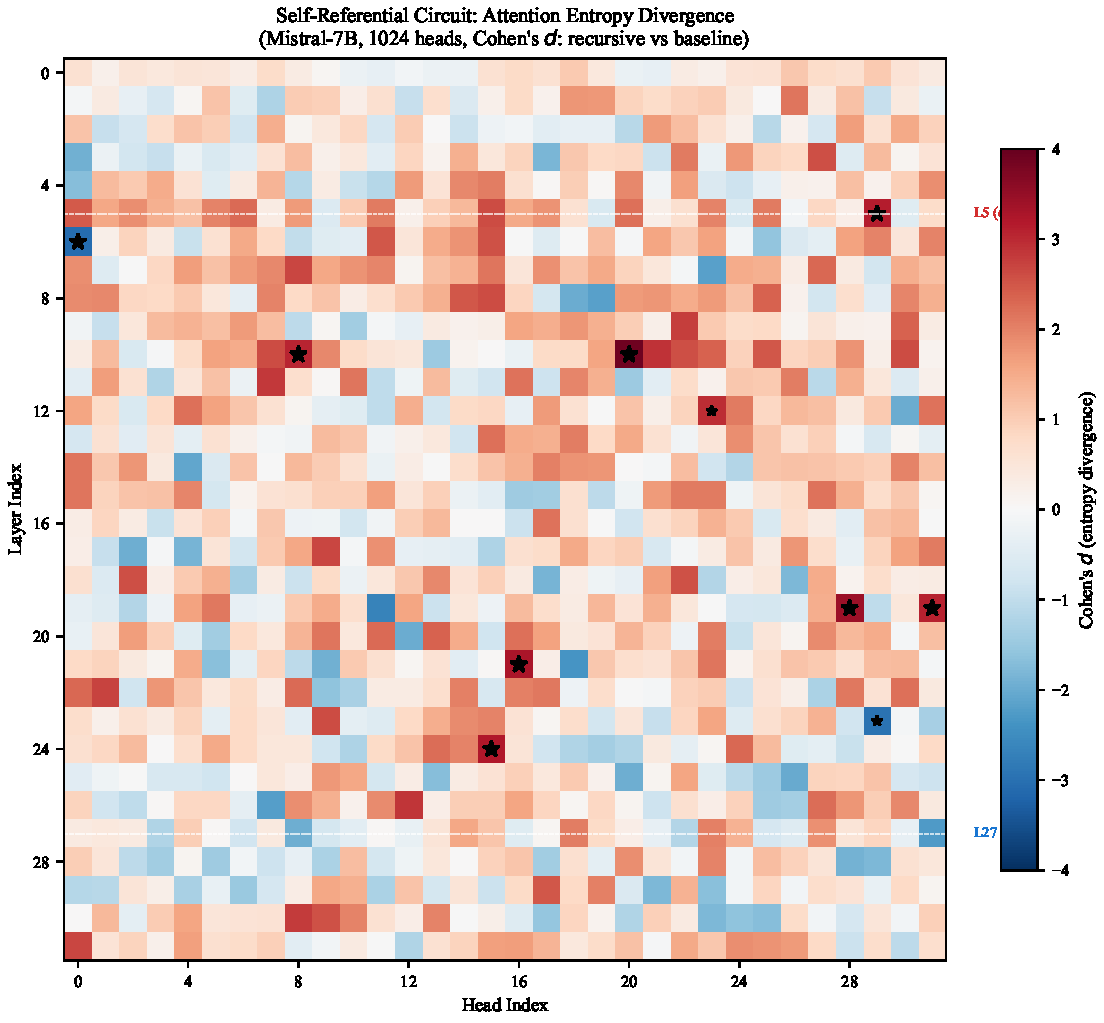
\includegraphics[width=0.95\linewidth]{fig_full_head_sweep_32x32.pdf}
\caption{\textbf{Full 32$\times$32 head sweep (Mistral-7B, $n = 100$ per condition).}
         Color encodes $\dcohen$ for entropy separation between recursive and baseline prompts.
         907 of 1{,}024 heads are significant on entropy
         ($p < 0.05$, uncorrected).}
\label{fig:head_sweep}
\end{figure}

\begin{table}[ht]
\centering
\caption{Top 10 attention heads by entropy separation in the refreshed base $n = 100$ head sweep.}
\small
\begin{tabular}{ccrr}
\toprule
Layer & Head & $\dcohen_\mathrm{entropy}$ & Significance \\
\midrule
20 & 09 & $+$3.43 & $p < 10^{-30}$ \\
22 & 08 & $+$3.37 & $p < 10^{-30}$ \\
24 & 14 & $+$3.30 & $p < 10^{-30}$ \\
21 & 16 & $+$3.17 & $p < 10^{-29}$ \\
21 & 22 & $+$3.17 & $p < 10^{-32}$ \\
24 & 15 & $+$3.11 & $p < 10^{-30}$ \\
26 & 16 & $+$3.09 & $p < 10^{-30}$ \\
17 & 30 & $+$3.09 & $p < 10^{-29}$ \\
23 & 27 & $+$3.06 & $p < 10^{-29}$ \\
22 & 30 & $+$3.06 & $p < 10^{-32}$ \\
\bottomrule
\end{tabular}
\end{table}


\section{Representation Analysis}
\label{app:representation}

\paragraph{Concept erasure.}
A logistic regression probe achieves 100\% accuracy classifying self-referential vs.\ baseline
from Layer~4 onward.
Projecting out this classification direction and recomputing $\RV$: the effect is unchanged
($\dcohen = -1.82$ before, $\dcohen = -1.82$ after; $\Delta d = 0.005$).
The geometric contraction operates in a \emph{different subspace} from the linear probe's
classification direction---$\RV$ is not reducible to a single discriminant axis.

\paragraph{Distributed interchange intervention.}
At L5, individual PCA dimensions show $\RV \approx 1.0$ (near baseline); the effect accumulates
only with the top-20 dimensions ($\RV = 2.184$).
At L27, \emph{every} individual PCA dimension shows $\RV \approx 0.41$ (strong contraction);
top-20 combined: $\RV = 0.324$, $\dcohen = -3.42$.
The late-layer contraction is a \emph{global geometric property}, not a feature localized
to specific rotated directions.

\paragraph{Vocabulary projections.}
SVD vocabulary projections of the first singular direction in L27H10 show high scores for
continuation/completion tokens and low scores for entity tokens, encoding a
\emph{continuation-vs-entity} gate.
L27H31's second singular direction encodes a literal \emph{self/other} axis:
top tokens are ``own'', ``Own'', ``answer'' while bottom tokens are ``same'', ``kind'', ``sorts''.


\section{SVD Circuit Taxonomy}
\label{app:svd_taxonomy}

\begin{table}[ht]
\centering
\caption{SVD decomposition of seven circuit heads in Mistral-7B ($n = 100$ per condition).}
\label{tab:svd_heads}
\small
\begin{tabular}{lcrrrl}
\toprule
Head & Role & $\dcohen_{\text{rank}}$ & $\dcohen_{\text{top1}}$ & Stability & SV1 Semantic Axis \\
\midrule
L27H10 & Compress & $-$1.32 & 1.36 & 0.94 / 0.54 & exploratory token axis \\
L27H2  & Compress & $-$1.35 & 1.51 & 0.90 / 0.79 & exploratory token axis \\
L27H26 & Compress & $-$0.95 & 0.45 & 0.20 / 0.34 & exploratory token axis \\
L5H29  & Diversify & $+$0.94 & $-$0.51 & 0.52 / 0.42 & exploratory token axis \\
L5H15  & Neutral & $-$0.02 & $-$0.14 & 0.60 / 0.43 & exploratory token axis \\
L27H18 & Compress & $-$0.74 & 0.84 & 0.70 / 0.30 & exploratory token axis \\
L27H31 & Neutral & $-$0.43 & 0.23 & 0.60 / 0.40 & exploratory token axis \\
\bottomrule
\end{tabular}
\vspace{1mm}

\raggedright\footnotesize
Role: Compress = rank contracts for recursive ($\dcohen < -0.5$);
Diversify = rank expands ($\dcohen > 0.5$);
Neutral = $|\dcohen| < 0.5$.
Stability: mean cosine similarity of top-1 singular vector across prompts (recursive / baseline).
The SV1 semantic axis column reports exploratory token-axis alignment; the locked claims are the numeric rank and stability values.
\end{table}


\section{Theoretical Framework}
\label{app:theory}

\subsection{Participation Ratio on the Grassmannian}

The singular value decomposition $\mathbf{A}^{(l)} = \mathbf{U} \boldsymbol{\Sigma} \mathbf{V}^\top$
associates to each activation a point on the Grassmannian $\text{Gr}(k, d)$ via the column space.
The participation ratio is a spectral functional of the Gram matrix
$\mathbf{G} = \mathbf{A}^\top \mathbf{A}$:
\begin{equation}
    \PR = \frac{(\text{tr}\,\mathbf{G})^2}{\text{tr}\,\mathbf{G}^2} = \frac{\|\boldsymbol{\lambda}\|_1^2}{\|\boldsymbol{\lambda}\|_2^2}
\end{equation}
where $\boldsymbol{\lambda}$ is the eigenvalue vector of $\mathbf{G}$.

\subsection{Random Matrix Theory Baseline}

Under the null hypothesis that activations are drawn i.i.d.\ from
$\mathcal{N}(0, \sigma^2 \mathbf{I})$, the eigenvalues follow the
Mar\v{c}enko-Pastur distribution with $\gamma = D/W$.
For $W = 16$, $D = 4096$: $\PR_\mathrm{MP} \approx 15.94$ (near $W$).
Observed recursive $\PR_\mathrm{late} \approx 5.8$ (Mistral-7B)---well below the random null,
indicating structured spectral organization.

\subsection{Information-Geometric Interpretation}

Define geometric complexity as $C(l) = \log \PR(l)$. Then:
\begin{equation}
    \log \RV = C(L_\mathrm{late}) - C(L_\mathrm{early})
\end{equation}
Negative $\log \RV$ means the network reduces geometric complexity across layers.
Self-referential content produces the strongest reduction: representing ``the system processing
this text'' requires fewer effective dimensions than representing external domains.


\end{document}
